\documentclass{standalone}

\usepackage{tikz}

\begin{document}
\Large
\begin{tikzpicture}
% \draw[help lines, black!30] (0,0) grid (12,12);
\foreach \a in 
    {(2,2), (2,6), (2,10)}
    {\node at \a {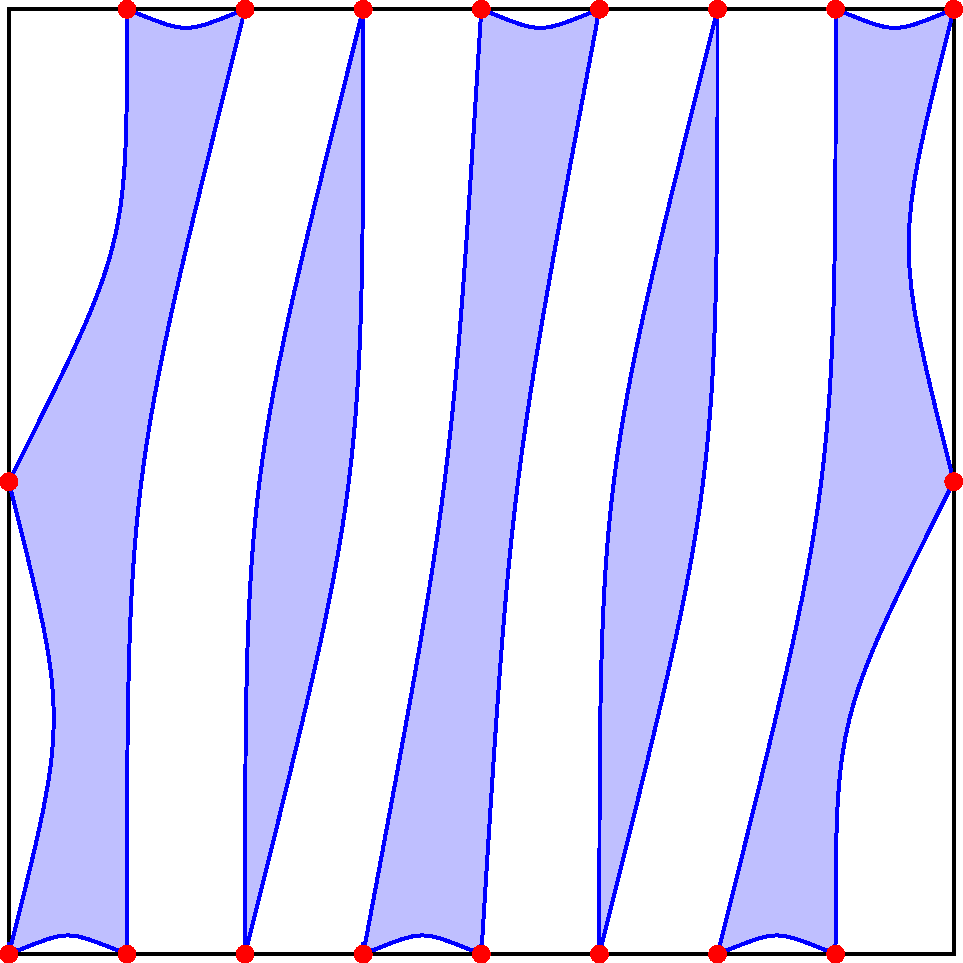
\includegraphics[width=4.1cm]{constr4clear.pdf}};};
\foreach \a in 
    {(6,0), (6,4), (6,8)}
    {\draw[line width=0.5mm, black!50] \a rectangle ++(4,4);
    \fill 
        \a++(2/3,2) circle (0.2)
        \a++(4/3,2) circle (0.2)
        \a++(2,2) circle (0.2)
        \a++(8/3,2) circle (0.2)
        \a++(10/3,2) circle (0.2);
        };
\foreach \a in 
    {(6,0), (6,4)}
    {\draw[line width=0.7mm]
        \a++(2/3,2) -- ++(0,4)
        \a++(2/3,2) -- ++(2/3,4)
        \a++(4/3,2) -- ++(2/3,4)
        \a++(2,2) -- ++(0,4)
        \a++(2,2) -- ++(2/3,4)
        \a++(8/3,2) -- ++(2/3,4)
        \a++(10/3,2) -- ++(0,4);
    };
\end{tikzpicture}
\end{document}